\section{Commands}
\label{sec:commands}

In the following we list all commands with the corresponding JSON schema.
For sake of synthesis, we indicate in a pretty custom way (pseudo-JSON) both the optional fields and the non primitive data types.

For example, in the following pseudo-JSON: \texttt{f1} is a mandatory field with value \texttt{v1}; \texttt{f2} is a mandatory field with domain in ad-hoc data type \texttt{T}; \texttt{f3} is an optional field with domain \texttt{T} and default value \texttt{default}; \texttt{f4} and \texttt{f5} are optional fields going together with domain \texttt{T} and default value \texttt{default}.

\begin{verbatim}
  {
    "f1": "v1",
    "f2": T,
    ("f3": T (default)),
    (
      "f4": T (default),
      "f5": T (default)
    )
  }
\end{verbatim}

In the command listed below there are non primitive data types. Some of them have been already mentioned in \ref{sec:configuration}. We report here them too, for reader's convenience.

\begin{description}
  \setlength\itemsep{1em}

  \item[time-expression] represents a temporal interval — e.g. a value in seconds between 3 and 5 seconds. This expression is a string in the form \texttt{min-max:unit}, where \texttt{min} is a positive long, \texttt{max} is a positive long greater than or equal to \texttt{min}, and \texttt{unit} is the string representation of a standard Java TimeUnit\footnote{i.e. NANOSECONDS, MICROSECONDS, MILLISECONDS, SECONDS, MINUTES, HOURS, DAYS.}. If \texttt{min} and \texttt{max} are both equal to a positive long \texttt{amount}, the time interval could be representaed both by the redundant expression \texttt{amount-amount:unit} and by the more compact expression \texttt{amount:unit}.
  For example, the following are valid expressions:

  \begin{verbatim}
    3-5:SECONDS

    10:SECONDS
  \end{verbatim}

  \item[proxy-expression] represents a HTTP proxy — e.g. the proxy 123.123.123.123 with port 3000. This expression is a string in the form \texttt{address:port}, where \texttt{addres} is an IPv4 address and \texttt{port} is a port number. The expression can also be a string \texttt{none}, meaning that no proxy should be used, and \texttt{null}, meaning that any default proxy should be used.
  For example, the following are valid expressions:

  \begin{verbatim}
    123.123.123:3000

    none
  \end{verbatim}

  \item[web-expression] represents a Web URL — http://www.google.com. Pay attention that it is necessary to specify the HTTP protocol.
  For example, the following is valid expressions:

  \begin{verbatim}
    http://www.google.com
  \end{verbatim}

  whereas the following is not

  \begin{verbatim}
    www.google.com
  \end{verbatim}

  \item[dict-object] represents a dictionary between strings and strings — e.g. "prop1" set to "val1".
  For example, the following is valid expressions:

  \begin{verbatim}
    {
      "prop1": "val1",
      "prop2": "val2"
    }
  \end{verbatim}

  \item[attack-object] represents a HTTP Flooding attack \cite{anderson2008security} — e.g. a POST attack to http://www.gmarciani.com.
  If specified, \texttt{proxy} is the HTTP proxy to attack through. If set to \texttt{null}, it is the default proxy (see \ref{sec:configuration}).
  If specified, \texttt{header} are the HTTP request header fields-value.
  If specified, \texttt{params} are the HTTP request data embedded into the URL when executing a GET attack, or encoded as \texttt{text/plain} when executing a POST attack.
  If specified, \texttt{executions} indicates how many attack executions need to be scheduled interleaved by the secified \texttt{period}.

  \begin{verbatim}
  {
    "method": value in [GET,POST],
    "target": web-expression,
    ("proxy": proxy-expression (null)),
    ("header": dict-object ({})),
    ("params": dict-object ({})),
    (
      "executions": integer in [1,65535] (1),
      "period": time-expression (null)
    )
  }
  \end{verbatim}

  For example, the following are valid expressions:

  \begin{verbatim}
  {
    "method": "GET",
    "target": "http://www.google.com"
  }

  {
    "method": "GET",
    "target": "http://www.google.com",
    "proxy": "123.123.123:3000",
    "header": {
      "User-Agent": "MyAwesomeBot",
      "Authentication": "Basic 123456789",
      "BotID": 270690
    },
    "executions": 3,
    "period": "3-5:SECONDS"
  }
  \end{verbatim}

  \item[controller-object] represents a controller — e.g. a controller with init interface X command interface Y and log interface Z. A controller is expressed in the following form:

  \begin{verbatim}
    {
      "init": resource-expression
      "cmd":  resource-expression
      "log":  resource-expression
      ("polling": time-expression),
      ("reconnections": integer in [0,65535] (0)),
      ("reconnectionWait": time-expression (null)),
      ("proxy": proxy-expression (null)),
      ("sleep": cron-expression (null)),
      ("authentication": dict-object ({}))
    }
  \end{verbatim}

  where a \texttt{resource-expression} represents a readable local or remote resource — i.e. a standard file pathname or a remote Web URL.

\end{description}

Every command starts with a \textit{timestamp}, a field pointing out the \textit{command scope}, and terminates with the expected \textit{parameters}.
Every command\footnote{with the exception of command \texttt{NONE} having no fields, and command \texttt{REPORT} having no optional field \texttt{report}.}  has a optional fields \texttt{delay} and \texttt{report}.

If \texttt{delay} is specified, the command will be executed after a random amount of time within the given interval; if not, the command will be executed immediately. This optional field has been added to command schema because in some real scenarios could be useful to specify a variance component.

If \texttt{report} is specified and set to \texttt{true}, the bot will send the report back to the controller, once the command has been executed. If set to \texttt{false}, no report will be sent back to the controller. This optional field has been added to the command schema as a shortcut for whichever command followed by the \texttt{REPORT} command. Sometimes, as stated in \cite{build-your-own-botnet}, the reporting procedure is embedded in every bot-controller interaction, as a bot response to command requests. We avoided such an approach because (i) it does not scale with botnet dimension\footnote{it would sound somehow as a DDoS suicide.} and (ii) the local host analysis is an action in itself, not strictly related to the curretn executing command\footnote{for example, keylogging is not a bot response to controller's requests, but an additional, though frequent, function.}.

\begin{description}
  \setlength\itemsep{1em}

  \item[ATTACK-HTTPFLOOD] schedules all the specified HTTP Flooding \texttt{attacks}.

  \begin{verbatim}
  {
    "timestamp": integer,
    "command": "ATTACK_HTTPFLOOD",
    "attacks": [ attack-object ],
    ("delay": time-expr (null))
  }
  \end{verbatim}

  \item[CALMDOWN] all attacks are unscheduled.
  If \texttt{wait} is true, it waits for for termination of currently executing attacks; if false, it kills them immediately.

  \begin{verbatim}
  {
    "timestamp": integer,
    "command": "CALMDOWN",
    ("wait": boolean (false)),
    ("delay": time-expr (null))
  }
  \end{verbatim}

  \item[KILL] the bot is killed, that is alla attacks are unscheduled and it transit to state \texttt{DEAD} for resource releasing.
  If \texttt{wait} is true, it waits for for termination of currently executing attacks; if false, it kills them immediately.

  \begin{verbatim}
  {
    "timestamp": integer,
    "command": "KILL",
    ("wait": boolean (false)),
    ("delay": time-expr (null))
  }
  \end{verbatim}

  \item[NONE] instructs the bot to do nothing, that is to neither change its executions flow nor send any report. In particular, both the null (empty file) and the empty command (empty JSON, i.e. {}) are equivalent to \texttt{NONE}.

  \begin{verbatim}
  {
    ("timestamp": integer),
    "command": "NONE"
  }
  \end{verbatim}

  \item[REPORT] the bot sends the report to the controller.

  \begin{verbatim}
  {
    "timestamp": integer,
    "command": "REPORT",
    ("delay": time-expr (null))
  }
  \end{verbatim}

  \item[RESTART] all attacks are unscheduled, the bot transits to state \texttt{INIT} trying to contact the controller with \texttt{resource} as its init-interface.
  If \texttt{wait} is true, it waits for for termination of currently executing attacks; if false, it kills them immediately.

  \begin{verbatim}
  {
    "timestamp": integer,
    "command": "RESTART",
    "resource": [ controller-object ],
    ("wait": boolean (false)),
    ("delay": time-expr (null))
  }
  \end{verbatim}

  \item[SLEEP] all attacks are suspended and the bot transits to state \texttt{SLEEP}. If a \texttt{timeout} si specified the command \texttt{WAKEUP} is internally invoked after a random amount of time within the specified interval.

  \begin{verbatim}
  {
    "timestamp": integer,
    "command": "SLEEP",
    ("timeout": time-expr (null)),
    ("delay": time-expr (null))
  }
  \end{verbatim}

  \item[UPDATE] the bot configuration is updated with the properties specified in \texttt{settings}. This command is tipically used to update the property \texttt{sleep} that sets the sleep mode.

  \begin{verbatim}
  {
    "timestamp": integer,
    "command": "UPDATE",
    "settings": map-expr,
    ("delay": time-expr (null))
  }
  \end{verbatim}

  \item[WAKEUP] if the bot is in state \texttt{SLEEP}, it lets scheduled attacks be able to fire again and transits to state \texttt{EXECUTION}.

  \begin{verbatim}
  {
    "timestamp": integer,
    "command": "WAKEUP",
    ("delay": time-expr (null))
  }
  \end{verbatim}

\end{description}

\subsection{Commands WUI}\label{sec:commands-wui}
The WUI, designed to give commands to the bot is divided into two sections: the bot operating activities and the attack command. The operating activities section includes the following commands: \textit{Kill}, \textit{Restart}, \textit{Report}, \textit{Sleep}, \textit{Wakeup} and \textit{Update}. As you can see in the figure \ref{fig:commands-wui}, a select box is used to define the desired activity. The choice of any command enables the associated options for that; for example the delay option for “Kill”. Other options that can be enabled are: "Report", for a response of command execution, and "Wait". The "Generate Command" button produces the JSON file for the configured activity.

\begin{figure}[tp]
  \centering
  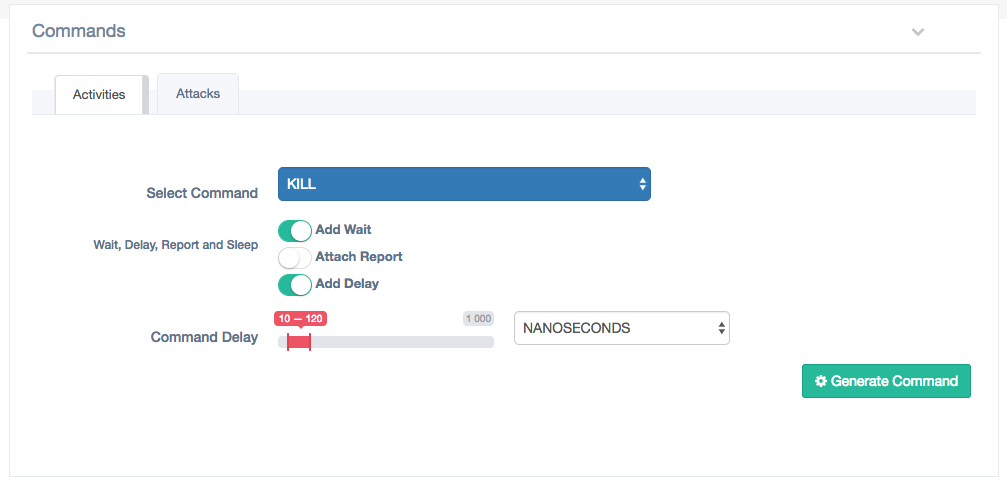
\includegraphics[scale=0.45]{./fig/commandsWUI.png}
  \caption{The Web User Interface to build commands.}
    \label{fig:commands-wui}
\end{figure}

As for the attack section, in this part of interface you can specify the list of targets on which to execute an HTTP Flooding Attack. For each target, on the corresponding modal in figure \ref{fig:target-wui}, can be defined the HTTP request method (GET or POST), a specific proxy, the http request header and params fields, the number of executions and the waiting period between an execution and the other.

\begin{figure}[tp]
  \centering
  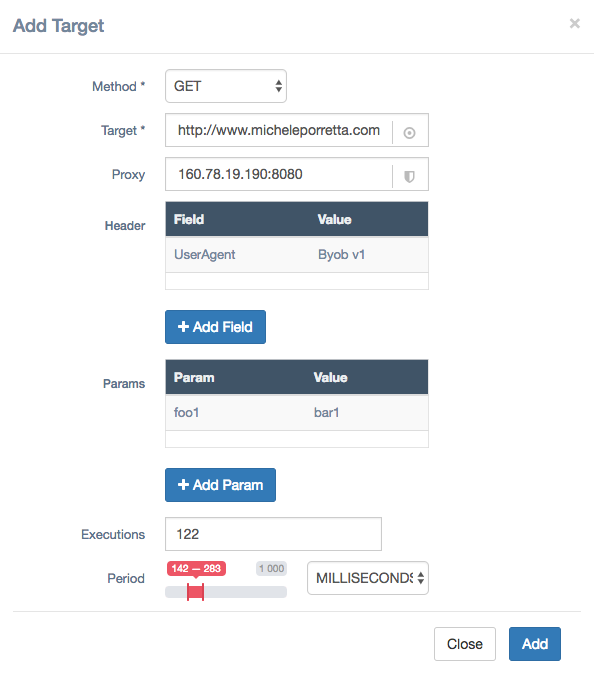
\includegraphics[scale=0.45]{./fig/targetWUI.png}
  \caption{The Web User Interface to define a target for attack}
    \label{fig:target-wui}
\end{figure}

After defining a list of attacks, can be associate the activation delay and enable a report of execution. Finally, the button "Generate Attack", it allows you to produce the JSON file with the attack's description, see \ref{fig:attack-wui};

\begin{figure}[tp]
  \centering
  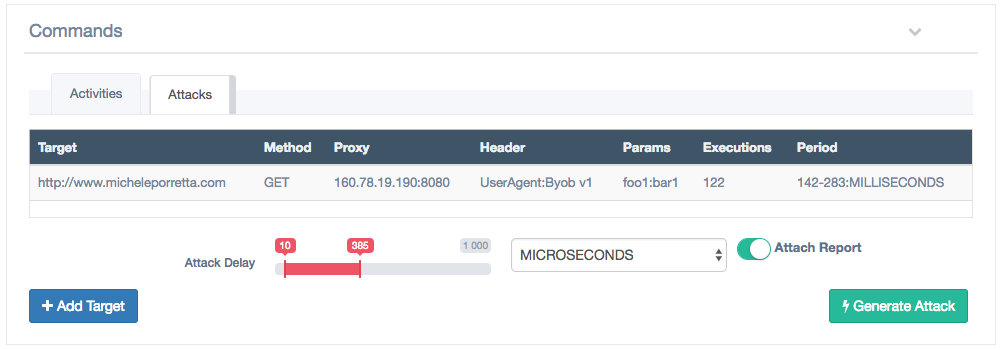
\includegraphics[scale=0.45]{./fig/attackWUI.png}
  \caption{The Web User Interface to define an HTTP Flooding Attack.}
    \label{fig:attack-wui}
\end{figure}
